\def\hnumber{2}
\def\student{Jerry Sun}
\def\studentid{ys7va}
\documentclass{cs4444}
\usepackage{tikz, pgfplots, graphicx}
\begin{document}

\maketitle

\section{Problem Description}
The goal of this assignment is to write a shell script to optimize the runtime for a film rendering problem. In particular, we want to explore the performance of converting a sequential program into a high-throughput implementation using SLURM on Rivanna.
	More specifically, the input file we are given is Star-collapse-ntsc.blend, and we are required to render 250 individual frames using blender. After that, we will need to use ffmpeg to combine those individual frames to output an avi file.  
\section{Metadata}
\subsection{Software}
	SLURM: version 14.11
	
	GNU bash: version 4.1.2
	
	blender: version 2.70
	
	ffmpeg: version 2.3.1

\subsection{Hardware}
	10 core Intel(R) Xeon(R) CPU E5-2670 v2 @ 2.50GHz with a cache size of 25600KB
	
\section{Approach}
	For this assignment, we are required to parallelized the whole film rendering process. There are two main process in this problem. First is the frame rendering process using blender, and the second is to combine individual frames. Since the second process can only work on a single node, so our main focus is on parallelizing the blender rendering process. 
	
	First, I modified the $slurm.sh$ using $srun$ to ensure all process are running in parallel, and added $-j$ $k$ flag in blender so now each single process will render each frame after jumping across k frames but only invoke $blender$ only one time(detail explanation see code comments in appendix). By doing this, the workload in different tasks can be distributed evenly, because based on testing, we found that the rendering later frames seem to be more time consuming than that of the earlier ones.
	
	Secondly, to automize the time testing based on number of process I use, I wrote $calculate.sh$ which will automatically submit $slurm.sh$ based on different number of processes, and record the time spent on each task correspondingly.
	
	Finally, to confirm that different partitioning method did give significantly different speedup, I wrote the $partition.sh$ to test a naive separate method, as I just evenly split the jobs into k parts and run all those tasks in parallel.
	
\section{Performance}
	In this section, I will give a brief analysis for the data I retrieved from the testing above.
	Since the clock time of the program running on Rivanna heavily depends on the load of the certain nodes that the task is assigned, there are various 'noisy' data during experiment, and those apparent outliers are eliminated when recorded.

\subsection{Runtime Analysis}
	Followed are all the inliers recorded during testing on Rivanna, and the average results for each number of tasks. Note that for all number of tasks smaller or equal to 20, all processes ran on different nodes, and for 40 tasks, they ran on 20 nodes, each got 2 tasks, and for 80 tasks all 20 nodes got 4 tasks.
\begin{center}
\begin{tabular}{ |c|c|c|c|c|c|c|c|c| }
\hline
iterations & 1 & 2 & 4 & 8 & 10 & 20 & 40 & 80 \\
\hline
 1st run & 401 & 203 & 105 & 55 & 42 & 29 & 20 & 25  \\ 
 2nd run & 400 & 201 & 100 & 57 & 46 & 27 & 17 & 19  \\ 
 3rd run & 402 & 198 & 103 & 58 & 46 & 29 & 21 & 20  \\
 4th run & 405 & 200 & 105 & 51 & 43 & 30 & 22 & 22  \\
 5th run & 406 & 199 & 107 & 52 & 45 & 28 & 21 & 22  \\
 6th run & 401 & 205 & 110 & 54 & 46 & 27 & 18 & 24  \\
 7th run & 399 & 205 & 104 & 59 & 49 & 27 & 20 & 19  \\
 8th run & 400 & 201 & 103 & 54 & 50 & 29 & 22 & 20  \\
 9th run & 405 & 200 & 100 & 54 & 44 & 30 & 17 & 23 \\
 10th run & 400 & 201 & 102 & 55 & 43 & 29 & 23 & 20 \\
 \hline
 average & 402 & 201 & 104 & 55 & 46 & 28 & 20 & 22  \\
 \hline
\end{tabular}
\end{center}
Followed is the comparison graph given the average results above. We can see it is almost exponentially decreasing at first but when reaching more than 20 nodes, the increase in speed seems to shrink really quickly. This is mainly due to the overhead caused by communication and imbalance work load in different tasks.
\begin{center}
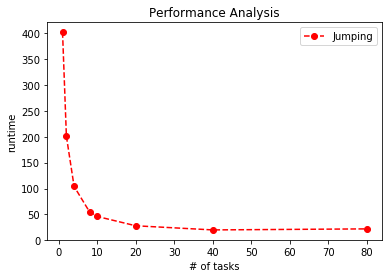
\includegraphics[width=12cm, height=8cm]{jumping}
\end{center}
\subsection{Efficiency Analysis}
Here we also introduce another metric in parallel computing that is the efficiency. The equation is given below.
\[
	\text{Efficiency} = \frac{\text{Sequential Execution Time}}{\text{Number of Processors}*\text{Parallel Execution Time}}
\]
And followed is the efficiency graph given the data above.
\begin{center}
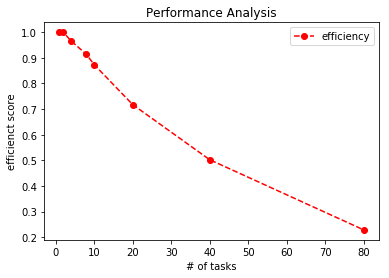
\includegraphics[width=12cm, height=8cm]{efficiency}
\end{center}
While we are looking for a high throughput strategy to faster the frame rendering process, we also want to keep the whole process relatively efficient. Therefore, based on the statistic above we would rather prefer 20 tasks in this particular problem to accelerate this process to avoid overhead as well as the efficiency loss.

\subsection{Partition Analysis}
 As mentioned at the beginning, we also want to see if the 'jumping strategy' is truly an efficient way to divide the whole task. Here we also experiment with a linear partitioning strategy in which each process works on approximately equal number of continuous frames. The test was only done for 20 tasks.
   \begin{center}
\begin{tabular}{ |c|c|c| }
\hline
 & jumping & linear \\
\hline
 1st run & 29 & 45 \\ 
 2nd run & 27 & 48 \\ 
 3rd run & 29 & 54 \\
 4th run & 30 & 60 \\
 5th run & 28 & 55 \\
 6th run & 27 & 56 \\
 7th run & 27 & 56 \\
 8th run & 29 & 49 \\
 9th run & 30 & 50 \\
 10th run & 29 & 50 \\
 \hline
 average & 28 & 53\\
 \hline
\end{tabular}
\end{center}
Therefore, we can see a clear gap between the jumping strategy and the linear partitioning strategy, which is mainly because of the uneven workload distributed in different tasks. 

\section{conclusion}
After the analysis above, we finally pick 20 tasks, and a so-called jumping strategy in parallelize this frame rendering process, which yields us a speedup ratio 14.3 and a efficiency score of 0.71. 
\section{Pledge}

\pledge
\newpage
\section{Appendix}
\subsection{calculate.sh}
\lstinputlisting[language=bash]{calculate.sh}
\newpage
\subsection{slurm.sh}
\lstinputlisting[language=bash]{slurm.sh}
\subsection{seq.sh}
\lstinputlisting[language=bash]{seq.sh}


\end{document}
